\documentclass{article}
\usepackage{amsmath}
\usepackage{mathtools}
\usepackage{gensymb}
\usepackage[a4paper,inner=1.5cm,outer=1.5cm,top=2cm,bottom=0.5cm]{geometry} 
\usepackage{xcolor}                    
\usepackage{tikz}                           
\usepackage{multicol}
\usepackage{hyperref}
\usepackage{pgfplots}
\usetikzlibrary{calc}
\usetikzlibrary{intersections}
\usetikzlibrary{intersections,calc,angles,quotes}
\usetikzlibrary{shapes,arrows,positioning,decorations.pathreplacing,calc}
\usetikzlibrary{calc,angles,positioning,intersections,quotes,decorations.markings}
\usepackage{tkz-euclide}
\usetikzlibrary{backgrounds}
\usetikzlibrary{calc,through}
\usetikzlibrary{angles}
\usetikzlibrary{fadings}
\usetikzlibrary{shapes.geometric}
\usetikzlibrary{shapes.symbols}
\usepackage{draftwatermark}
\usepackage{mathptmx}

\SetWatermarkText{\textcolor{black!20}{Mathema Shukur}}
\SetWatermarkFontSize{2 cm}
\usepackage[utf8]{inputenc}
\usepackage{fontspec}

\setmainfont{[Kalpurush.ttf]}
\newfontface{\en}{[Arial.ttf]} %%this is optional, if you want to use a secondary font. Any english font is supported
\newlength\Radius
\setlength\Radius{4cm}
\begin{document} 
	\Large
	\textcolor{red}{Welcome To} 
	\\
	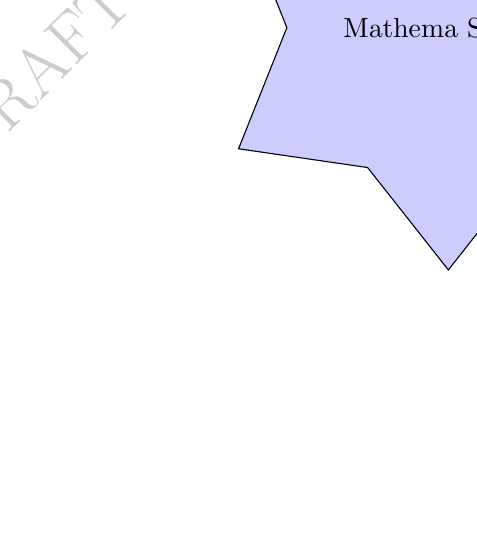
\begin{tikzpicture}
		\tikz \node [fill=blue!20,star,star points=6,draw] {Mathema Shukur };
	\end{tikzpicture}
	\\
	যাদের জন্যে প্রযোজ্যঃ  	\textcolor{magenta}{একাদশ ও দ্বাদশ শ্রেণীর শিক্ষার্থী} \\
	বিষয়ঃ \textcolor{magenta}{উচ্চতর গণিত ১ম পত্র} \\
	অধ্যায়ঃ \textcolor{magenta}{৪-বৃত্ত}\\ 
	\\
	\\
	\href{https://www.youtube.com/watch?v=DRxNte3mU6U&list=PLIjPH8h-K22w5iYZogyV1AI8-baSpY2Qn&index=1}{\textcolor{blue}{মূল বিন্দুতে (0,0) কেন্দ্র থাকলে বৃত্তের সমীকরণ কী?}}\\
	\\
	\href{https://www.youtube.com/watch?v=rGCA1MltZsY&list=PLIjPH8h-K22w5iYZogyV1AI8-baSpY2Qn&index=2}{\textcolor{blue}{কী শর্তে কেন্দ্রের স্থানাঙ্ক হতে বৃত্তের ব্যাসার্ধ নির্ণয় করা হয়?}}\\
	\\
	\href{https://www.youtube.com/watch?v=gehIW-_0XrQ&list=PLIjPH8h-K22w5iYZogyV1AI8-baSpY2Qn&index=3}{\textcolor{blue}{বৃত্তের সাধারণ সমীকরণ $x^2+y^2+2gx+2fy+c=0$}}\\
	\\
	\href{https://www.youtube.com/watch?v=WzuG-MuA6Cs&list=PLIjPH8h-K22w5iYZogyV1AI8-baSpY2Qn&index=4}{\textcolor{blue}{পোলার স্থানাঙ্কে বৃত্তের সমীকরণ নির্ণয়}}\\
	\\
	\href{https://www.youtube.com/watch?v=ssCuBx7HEHI&list=PLIjPH8h-K22w5iYZogyV1AI8-baSpY2Qn&index=5}{\textcolor{blue}{ব্যাসের প্রান্ত বিন্দু (x1,y1) ও (x2,y2) হলে বৃত্তের সমীকরণ নির্ণয়}}\\
	\\
	\href{https://www.youtube.com/watch?v=afVjGQrIpDs&list=PLIjPH8h-K22w5iYZogyV1AI8-baSpY2Qn&index=6}{\textcolor{blue}{বৃত্ত ও সরলরেখার ছেদবিন্দুগামী বৃত্তের সমীকরণ}}\\
	\\
	\href{https://www.youtube.com/watch?v=rXOyjYE6YfU&list=PLIjPH8h-K22w5iYZogyV1AI8-baSpY2Qn&index=7}{\textcolor{blue}{দুইটি বৃত্তকে ছেদ করে এমন বৃত্তের সমীকরণ}}\\
	\\
	\href{https://www.youtube.com/watch?v=iQIWTRqZsAY}{\textcolor{blue}{৩ টি বিন্দুগামী বৃত্তের সমীকরণ নির্ণয়}}\\
	\\
	\vspace{2cm}
	\\
	\textcolor{magenta}{২ টি বৃত্ত পরস্পরকে স্পর্শ করার শর্ত }\\
	\\
	\vspace{2cm}
	\\
\textcolor{blue}{	দুইটি বৃত্ত পরস্পরকে বহিঃস্থ ভাবে স্পর্শ করলে কেন্দ্রদ্বয়ের দূরত্ব= ব্যাসার্ধদ্বয়ের যোগফল অর্থাৎ $C_1C_2=r_1+r_2$ হবে। }
	\\
	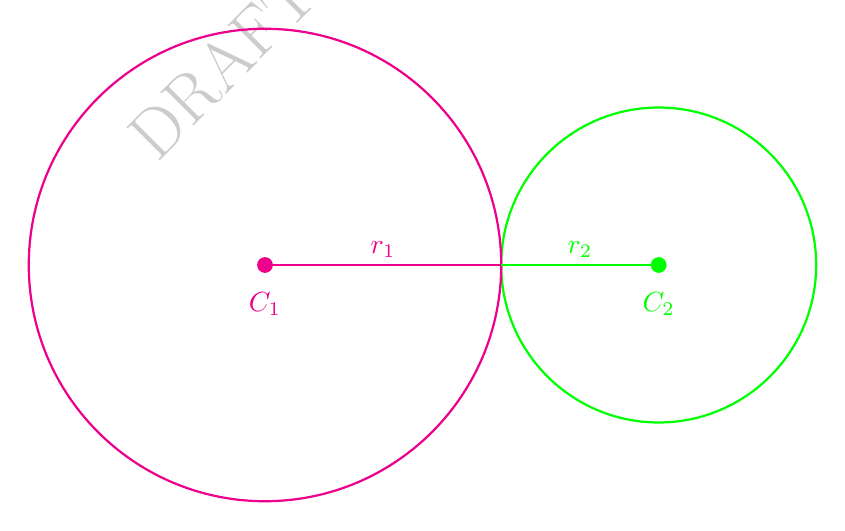
\begin{tikzpicture}[transform shape,scale=1]
		\draw[thick,green] (2,3) circle (2);
			\node at (2,2.5) {$\textcolor{green}{C_2}$};
			\node at (1,3.2) {$\textcolor{green}{r_2}$};		
		\fill[green] (2,3) circle (1 mm);
			\draw[thick,magenta] (-3,3) circle (3);
		\node at (-3,2.5) {$\textcolor{magenta}{C_1}$};	
		\node at (-1.5,3.2) {$\textcolor{magenta}{r_1}$};			
		\fill[magenta] (-3,3) circle (1 mm);
		\draw[magenta](-3,3)--(0,3);
			\draw[green](2,3)--(0,3);
	\end{tikzpicture}\\
\\ 
	\textcolor{red}{[ঢাকা বোর্ড-২০১৯]}\\ 
দেখাও যে, $x^2+y^2=36$ এবং $x^2+y^2+20x+84=0$ বৃত্তদ্বয় পরস্পরকে বহিঃস্থ ভাবে স্পর্শ করে। \\
\begin{align*}
	x^2+y^2&=36\\
	\\
	(x-0)^2+(y-0)^2&=6^2
\end{align*}
১ম বৃত্তের কেন্দ্র $C_1(0,0)$ ও ব্যাসার্ধ  $r_1=6$\\
\begin{align*}
	x^2+y^2+20x+84&=0\\
	\\
	x^2+y^2+2(10)x+2(0)y+84&=0
\end{align*}
২য় বৃত্তের কেন্দ্র $(-g,-f)=C_2(-10,0)$  ও ব্যাসার্ধ $\sqrt{g^2+f^2-c}=\sqrt{(10)^2+(0)^2-84}=4=r_2$\\
\\ 
কেন্দ্রদ্বয়ের মধ্যবর্তী দূরত্ব  $C_1C_2=\sqrt{(0+10)^2+(0-0)^2}=10$\\ 
\\
ব্যাসার্ধদ্বয়ের যোগফল
$r_1+r_2=6+4=10$\\
\\ 
যেহেতু কেন্দ্রদ্বয়ের মধ্যবর্তী দূরত্ব ব্যাসার্ধদ্বয়ের যোগফলের সমান সেহেতু বৃত্তদ্বয় পরস্পরকে বহিঃস্থ ভাবে স্পর্শ করে। \\
\\
\vspace{5cm} 
	\\
	\textcolor{blue}{দুইটি বৃত্ত পরস্পরকে অন্তঃস্থ ভাবে স্পর্শ করলে কেন্দ্রদ্বয়ের দূরত্ব= ব্যাসার্ধদ্বয়ের বিয়োগফলের পরম মান অর্থাৎ $C_1C_2=|r_1-r_2|$ হবে। }	\\
	\\
		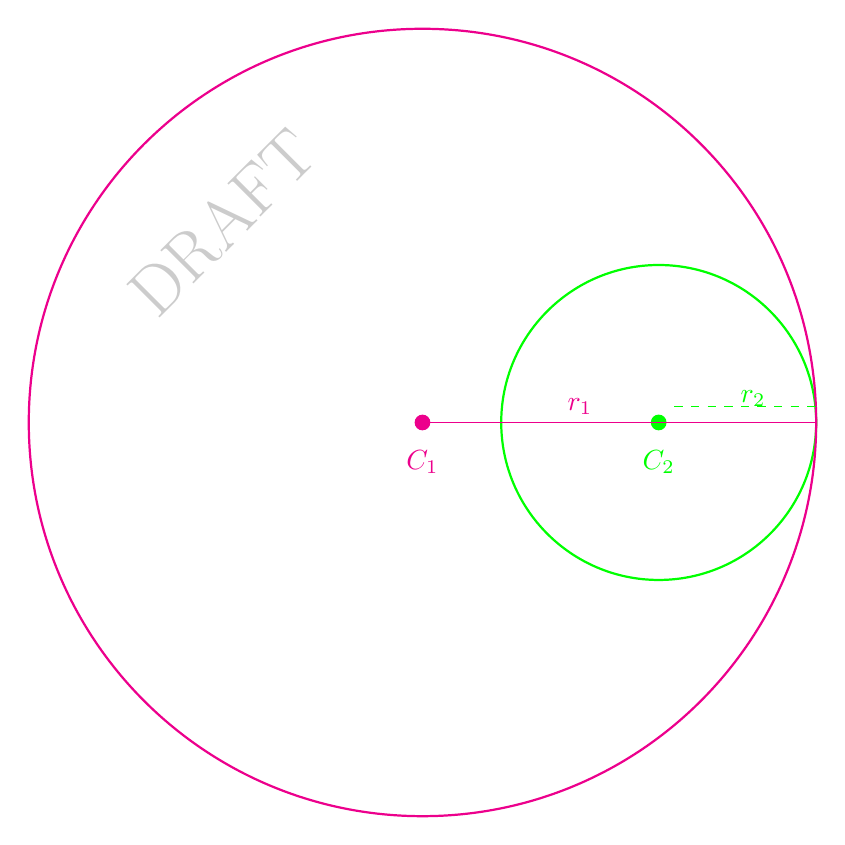
\begin{tikzpicture}[transform shape,scale=1]
		\draw[thick,green] (3,3) circle (2);
		\node at (3,2.5) {$\textcolor{green}{C_2}$};
		\node at (4.2,3.3) {$\textcolor{green}{r_2}$};		
		\fill[green] (3,3) circle (1 mm);
		\draw[thick,magenta] (0,3) circle (5);
		\node at (0,2.5) {$\textcolor{magenta}{C_1}$};	
		\node at (2,3.2) {$\textcolor{magenta}{r_1}$};			
		\fill[magenta] (0,3) circle (1 mm);
		\draw[magenta](0,3)--(5,3);
		\draw[green,dashed](3.2,3.2)--(5,3.2);
	\end{tikzpicture}\\
\\
	\textcolor{red}{[বরিশাল বোর্ড-২০১১]}\\ 
দেখাও যে, $x^2+y^2-2x+4y-31=0$ এবং $x^2+y^2+4x-4y+7=0=0$ বৃত্তদ্বয় পরস্পরকে অন্তঃস্থ ভাবে স্পর্শ  করে । \\
\begin{align*}
x^2+y^2-2x+4y-31&=0\\
\\
x^2+y^2+2(-1)x+2(2)y+(-31)&=0
\end{align*}
\\
১ম বৃত্তের কেন্দ্র $(-g,-f)=C_1(1,-2)$ ও ব্যাসার্ধ  $\sqrt{(-1)^2+(-2)^2-(-31)}=6=r_1$\\
\\ 
\begin{align*}
x^2+y^2+4x-4y+7&=0\\
	\\
	x^2+y^2+2(2)x+2(-2)y+(7)&=0
\end{align*}
\\
২য় বৃত্তের কেন্দ্র $(-g,-f)=C_2(-2,2)$ ও ব্যাসার্ধ  $\sqrt{(2)^2+(-2)^2-(7)}=1=r_2$\\
\\ 
কেন্দ্রদ্বয়ের মধ্যবর্তী দূরত্ব  $C_1C_2=\sqrt{(1+2)^2+(-2-2)^2}=5$\\ 
\\
ব্যাসার্ধদ্বয়ের বিয়োগফলের পরম মান $|r_1-r_2|=|6-1|=5$\\
\\ 
যেহেতু কেন্দ্রদ্বয়ের মধ্যবর্তী দূরত্ব ব্যাসার্ধদ্বয়ের বিয়োগফলের পরম মান সমান সেহেতু বৃত্তদ্বয় পরস্পরকে অন্তঃস্থ ভাবে স্পর্শ  করে । \\
\\
	\textcolor{red}{[রাজশাহী বোর্ড-২০১৭]}\\ 
দেখাও যে, $x^2+y^2+6x+8y+21=0$ এবং  $x^2+y^2=9$ বৃত্তদ্বয় পরস্পরকে  $\left(-\frac{9}{5},-\frac{12}{5}\right)$ বিন্দুতে বহিঃস্থ ভাবে স্পর্শ করে। \\
\\ 
\begin{align*}
x^2+y^2+6x+8y+21&=0\\
\\
x^2+y^2+2(3)x+2(4)y+21&=0\\
\end{align*}
\\ 
১ম বৃত্তের কেন্দ্র $(-g,-f)=C_1(-3,-4)$ ও ব্যাসার্ধ  $\sqrt{(-3)^2+(-4)^2-21}=2=r_1$\\
\\
\begin{align*}
x^2+y^2&=9\\ 
	\\
(x-0)^2+(y-0)^2&=3^2\\
\end{align*}
\\ 
২য় বৃত্তের কেন্দ্র $C_2(0,0)$ ও ব্যাসার্ধ  $r_2=3$\\
\\ 
\\ 
কেন্দ্রদ্বয়ের মধ্যবর্তী দূরত্ব  $C_1C_2=\sqrt{(-3-0)^2+(-4-0)^2}=5$\\ 
\\
ব্যাসার্ধদ্বয়ের যোগফল $r_1+r_2=2+3=5$\\
\\ 
যেহেতু কেন্দ্রদ্বয়ের মধ্যবর্তী দূরত্ব ব্যাসার্ধদ্বয়ের যোগফলের সমান সেহেতু বৃত্তদ্বয় পরস্পরকে বহিঃস্থ ভাবে স্পর্শ করে। \\
\\ 
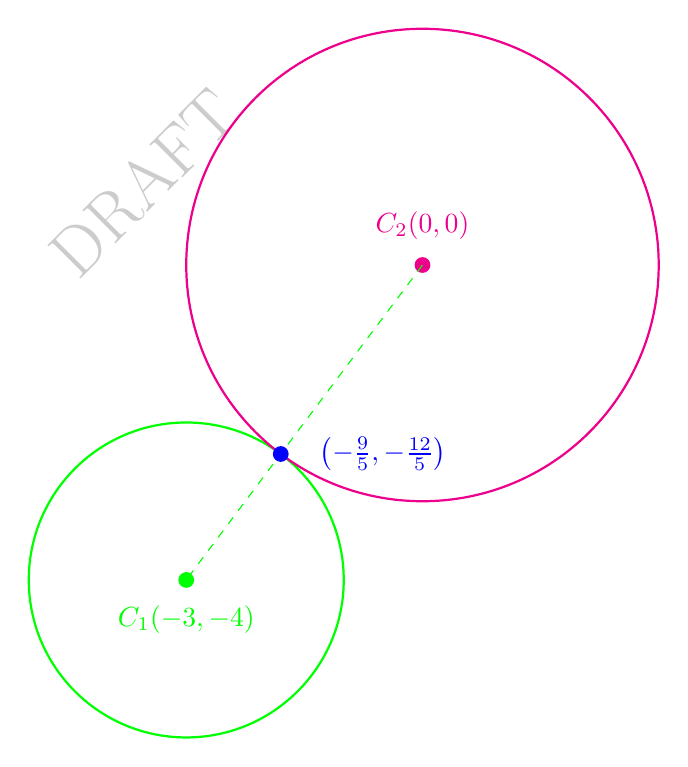
\begin{tikzpicture}[transform shape,scale=1]
	\draw[thick,green] (-3,-4) circle (2);
	\node at (-3,-4.5) {$\textcolor{green}{C_1(-3,-4)}$};
	\fill[green] (-3,-4) circle (1 mm);
	\draw[thick,magenta] (0,0) circle (3);
	\node at (0,0.5) {$\textcolor{magenta}{C_2(0,0)}$};		
	\fill[magenta] (0,0) circle (1 mm);
	\draw[green,dashed](0,0)--(-3,-4);
	\fill[blue] (-1.8,-2.4) circle (1 mm);
		\node at (-0.5,-2.4) {$\textcolor{blue}{\left(-\frac{9}{5},-\frac{12}{5}\right)}$};
\end{tikzpicture}\\
\\
স্পর্শ বিন্দুর স্থানাংকঃ ( অন্তর্বিভক্তকারী সেকশন ফর্মুলা ব্যবহার করি)\\ 
\\ 
 ধরি, $C_1(-3,-4)$ ও $C_2(0,0)$ বিন্দুর সংযোজক সরলরেখার $2:3$ অনুপাতে অন্তর্বিভক্তকারী বিন্দু $(x,y)$ হলো স্পর্শ বিন্দু ।\\
 \\
 $x_1=-3$,\,\,\,\ $x_2=0$,\,\,\,\  $y_1=-4$, \,\,\,\ $y_2=0$\\
 \\
 $r_1=2$,\,\,\,\ $r_2=3$\\
 \\   
 \begin{align*}
 	x&=\frac{r_1x_2+r_2x_1}{r_1+r_2}\\
 	\\
 	&=\frac{(2)(0)+(3)(-3)}{2+3}\\
 	\\
 	&=-\frac{9}{5}
 \end{align*}
\\   
\begin{align*}
	y&=\frac{r_1y_2+r_2y_1}{r_1+r_2}\\
	\\
	&=\frac{(2)(0)+(3)(-4)}{2+3}\\
	\\
	&=-\frac{12}{5}
\end{align*}
স্পর্শ বিন্দুর স্থানাংক $\left(-\frac{9}{5},-\frac{12}{5}\right)$ \\
\\ 
একটি বৃত্তের সমীকরণ নির্ণয় কর যার কেন্দ্রের স্থানাঙ্ক $(4,3)$  এবং যা $x^2+y^2=4$ বৃত্তকে বহিঃস্থ ভাবে স্পর্শ করে। \\
\\
১ম বৃত্তের কেন্দ্র $C_1(4,3)$ ও ব্যাসার্ধ $r_1$
\\
\begin{align*}
x^2+y^2&=4\\
\\
(x-0)^2+(y-0)^2&=2^2
\end{align*}
\\
২য় বৃত্তের কেন্দ্র $C_2(0,0)$ ও ব্যাসার্ধ  $r_2=2$\\
\\ 
কেন্দ্রদ্বয়ের মধ্যবর্তী দূরত্ব  $C_1C_2=\sqrt{(4-0)^2+(3-0)^2}=5$\\ 
\\
ব্যাসার্ধদ্বয়ের যোগফল $r_1+r_2=r_1+2$\\
\\
\textcolor{blue}{	দুইটি বৃত্ত পরস্পরকে বহিঃস্থ ভাবে স্পর্শ করলে কেন্দ্রদ্বয়ের দূরত্ব= ব্যাসার্ধদ্বয়ের যোগফল অর্থাৎ $C_1C_2=r_1+r_2$ হবে। }\\
\\
\begin{align*}
	r_1+r_2&=C_1C_2\\
	\\
	r_1+2&=5\\
	\\
	r_1&=5-2\\
	\\
	r_1&=3
\end{align*}
\\
১ম বৃত্তের কেন্দ্র $C_1(4,3)$ ও ব্যাসার্ধ $r_1=3$
\begin{align*}
	(x-4)^2+(y-3)^2&=3^2\\
	\\
	x^2-8x+16+y^2-6y+9&=9\\
	\\
	x^2+y^2-8x-6y&=0
\end{align*}
\\ 
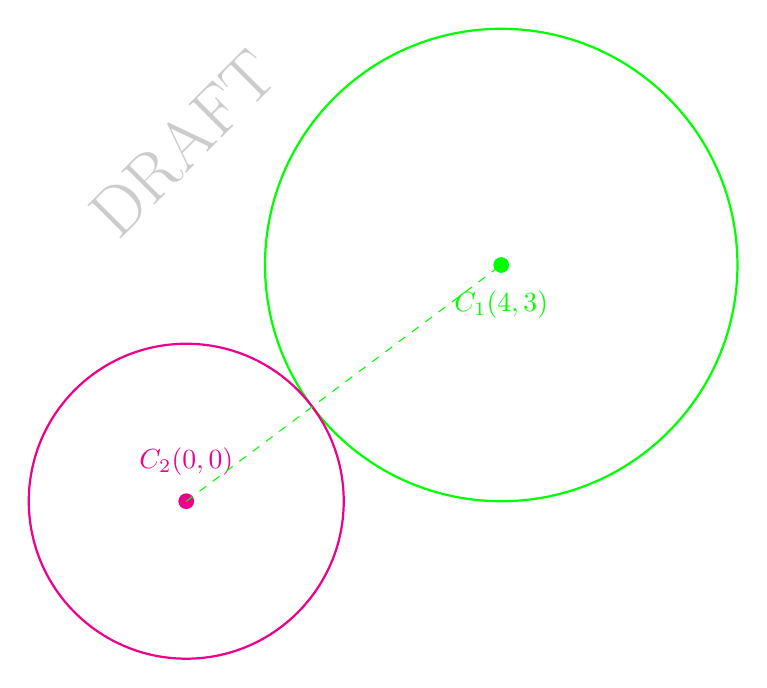
\begin{tikzpicture}[transform shape,scale=1]
	\draw[thick,green] (4,3) circle (3);
	\node at (4,2.5) {$\textcolor{green}{C_1(4,3)}$};
	\fill[green] (4,3) circle (1 mm);
	\draw[thick,magenta] (0,0) circle (2);
	\node at (0,0.5) {$\textcolor{magenta}{C_2(0,0)}$};		
	\fill[magenta] (0,0) circle (1 mm);
	\draw[green,dashed](0,0)--(4,3);
\end{tikzpicture}\\
\end{document}